\subsection{Flat boundary estimates: the cylinder loss}\label{c4:boundary-loss}

Our aim is to obtain spatial estimates for critical paths whose endpoints
lie on straight lattice cuts. A port is the midpoint of an edge crossing
such a cut. A path between ports visits vertices in the open domain, and
its weight is
\[
                     w(\gamma)=x_*^{L(\gamma)},\qquad
                x_*=(2+\sqrt2)^{-1/2},
\]
where $L(\gamma)$ counts visited vertices. Thus gluing at a port multiplies
weights exactly. In this section all arch masses use this convention.
Distances along a straight cut are measured in port spacings; Euclidean
and lattice distances differ only by fixed factors.

Let $h_n$ be the total weight of half-plane paths from a fixed boundary
port to the port $n>0$ spacings to its right. We shall prove
\begin{theorem}[Flat boundary arches]\label{a:flat-boundary}\label{thm:boundary-arches}
There are absolute constants $c,C>0$ such that, for every integer $n\ge1$,
\begin{equation}\label{c4:BA}
 \sum_{n\ge1}h_n=h_*:=\frac1{2\cos(3\pi/8)},\qquad
 c n^{-5/4}\le h_n\le C n^{-5/4},\qquad
 h_n[\operatorname{diam}\le Cn]\ge c n^{-5/4}.
\end{equation}
The total mass from a fixed port to any other port of its boundary line,
restricted to paths of diameter greater than $R$, is at most $CR^{-1/4}$
for $R\ge1$.
\end{theorem}
The exponent $5/4$ agrees with the boundary prediction from the
conjectural scaling picture of Lawler, Schramm and Werner, recorded
in~\cite[Section~4]{DuminilCopinSmirnov2012}.
The proof separates two questions. First we compute how much arch mass
is lost when the half-plane is wrapped onto a cylinder of circumference
$N$. This loss is of order $N^{-1/4}$. Then a three-root boundary identity
converts that loss into pointwise estimates and spatial confinement.

\subsubsection{An exact expression for the cylinder arch mass}
We use the $p=1$ vacuum constructed in Section~\ref{c4:vacua}, at
$q=Q^2=e^{i\pi/4}$ and twist $\eta=-i=q^{-2}$. Only even
circumferences are needed here. The polynomial tensor $V_N$ is the raw
vacuum; its empty component is $D=D_1$, and the physical stationary
state is $V_N/D$.

For an arc at ordered endpoints $i<j$, the link-map coefficient is
$q^{s_i}$ for either winding class. Thus the link diagrams may be read
as noncrossing diagrams in a disk. Write the component of the raw
$V_N$ supported just at $i,j$ as $q^{s_i}T_{ij}$, where $s_j=-s_i$.
Define the normalized scalar
\[
 F_N:=D^{-1}\sum_{i<j}z_i z_jT_{ij},\qquad t_i=z_i^2,
 \qquad \mathbf t=(t_i)_i.
\]
We shall prove the rational identity
\begin{equation}
 F_N=h_*\left[\sum_i t_i+\mathbf t^t\mathcal K^{-1}\mathbf1\right],
 \qquad
 \mathcal K_{ij}=\frac{t_i^2-t_j^2}{t_i^2+\sqrt2t_it_j+t_j^2}.
 \label{c4:BC}
\end{equation}
The main step is to prove that $F_N$ is symmetric in the site variables.
A null identity for the vacuum gives this symmetry; the even Pfaffian
formula of Section~\ref{c4:pair-denominator} then determines the scalar
by interpolation.

\paragraph{A covariant raising operator.}
Put $\kappa=Q^6$ and $K|s\rangle=\kappa^s|s\rangle$. Let $e$ raise
spin by one, with coefficients $Q^{-3},1,0$ from $-,0,+$, respectively,
and set
\[
 \mathcal E(z)=\sum_j z_jK_1\cdots K_{j-1}e_j.
\]
Charge conservation and the local identity
\[
 B(r)(r e\otimes I+K\otimes e)
       =(e\otimes I+r K\otimes e)B(r)
\]
make $\mathcal E$ covariant under exchange. To check the local identity,
use the tensors of Section~\ref{c4:local-tensors}. After multiplication
by $r^2g(x)$, $r=e^{ix}$, every entry of its difference is a polynomial
of degree at most five. It vanishes at $r=1,Q^3$; at the second point,
\[
 (e\otimes I+Q^3K\otimes e)C=0,\qquad
 C^t(Q^3e\otimes I+K\otimes e)=0.
\]
The negatives of these points are also roots by spin parity, since
conjugating $e$ by spin parity negates it. The constant term vanishes:
the limiting weighted swap intertwines $K\otimes e$ with $e\otimes I$
because $\xi\kappa=1$, and the extra term supported on
$|+,-\rangle\langle+,-|$ contributes zero on both sides. The reversed
swap at infinity similarly intertwines $e\otimes I$ with $K\otimes e$,
so the degree-five coefficient vanishes. The remaining degree-four
polynomial has the five roots just listed and is zero.

\paragraph{The null identity.}
We claim that $\mathcal E(z)^2V_N=0$. This tensor exchanges covariantly
and rotates with trivial twist. Indeed, for two raises with site
multiplicities $n_i$ summing to two, the order-dependent input phase is
\[
 \kappa^{\sum_i n_i\sum_{j<i}s_j};
\]
for distinct raised sites there is also the constant $1+\kappa$.
Left rotation subtracts $2s_1$ from the exponent on charge-zero inputs,
which is compensated by $\eta^{s_1}=\kappa^{2s_1}$.

At an adjacent positive fusion $z_j=Q^3z_i$, the inserted $C$ is neutral
and is killed by its local two-site raising sum. Induction on the
remaining sites therefore proves the null identity on this slice,
starting with the empty list (the one-site vacuum is killed as well).
Exchange and rotation give vanishing at both pair ratios
$t_j=q^{\pm3}t_i$ for any two sites. After stripping the output-spin
factors, every entry has degree at most $N-1$ in each $t_i$:
an extra power of $t_i$ can arise only from input spin $-$, whose
vacuum degree bound is $N-2$. The $2(N-1)$ pair roots prove the claim
for $N\ge2$.

\paragraph{Symmetry of the arc scalar.}
Take the component of this null identity with output $+,+$ at $1,2$
and vacancies elsewhere. For $2<l<m$, let $Z_{lm}$ be the raw diagram
weight with just the arcs $1m,2l$; equivalently it is the corresponding
$++--$ coefficient divided by $q^2$. Enumerating the raised sites and
dividing by $1+\kappa$ gives
\[
 0=D z_1z_2-h_*(t_1+t_2)T_{12}
   +\sum_{l>2}z_l(Q^{11}z_2T_{1l}+Q^5z_1T_{2l})
   +\sum_{2<l<m}z_lz_mZ_{lm}.
\]
For example, a double raise contributes $Q^{-3}/(1+\kappa)$ times its
diagonal spectral and prefix factors. Two exterior raises require
input $++--$ and multiply its arc phase by $\kappa^3Q^{-6}$.

On exchanging sites $1,2$, the coefficients change by
\[
 \begin{aligned}
 T_{12}&\longmapsto UD+wT_{12},\\
 \binom{T_{1l}}{T_{2l}}&\longmapsto
       (uI+v\,\mathrm{Swap})\binom{T_{1l}}{T_{2l}},\\
 T_{lm}&\longmapsto T_{lm}+UZ_{lm}.
 \end{aligned}
\]
In the last formula, closing $12$ kills a loop, while the nested arcs
join. The change of $DF_N$ is consequently $U$ times the displayed
null component: the needed local scalar equalities, with
$z_1/z_2=e^{ix}$, are
\[
 (v-1)e^{\pm ix}+u=-UQ^{\pm3},\qquad
 (1-w)z_1z_2=Uh_*(t_1+t_2),
\]
which follow by sine addition. Rotation preserves $F_N$, so all
adjacent exchanges preserve it. Thus $DF_N$ is symmetric and
polynomial in the $t_i$ before division by $D$.

\paragraph{Determination by pair fusion.}
The even Pfaffian formula for $D$ in Section~\ref{c4:pair-denominator}
shows that $D\,\mathbf t^t\mathcal K^{-1}\mathbf1$ is symmetric
polynomial of degree at most $N$ in each variable. Here the Pfaffian
cofactors clear kernel poles with the prefactor, and alternation gives
the required Vandermonde divisibility. The polynomial
$D(F_N-h_*\sum_i t_i)$ has the same degree bound.

Place a fused pair adjacent with $t_j=q^3t_i$. The vacuum prescription
makes $F_N$ equal its value on the shorter list plus
$Q^3t_i=h_*(t_i+t_j)$. Meanwhile $\mathcal K_{ij}$ has a pole, with
unrelated entries regular, so its inverse contraction reduces to that
on the shorter list. Symmetry gives the reversed pair ratio too.
Inductively, the difference between the two sides of
\eqref{c4:BC}, after clearing $D$, therefore vanishes at
$2(N-1)>N$ pair nodes for $N\ge4$. The initial case is
$F_2=h_*^{-1}t_1t_2/(t_1+t_2)$, from the two-site vacuum.
This proves \eqref{c4:BC}.

\subsubsection{The size of the homogeneous correction}
The exact formula reduces the cylinder loss to one scalar. Write
\(m_N\) for the homogeneous limit of \(\mathbf t^t\mathcal K^{-1}\mathbf1\). For \(N=2l\),
\begin{equation}
                         -m_N\asymp N^{3/4}.                       \label{c4:BM}
\end{equation}
In log-coordinates the kernel is \(\sinh w/(\cosh w+1/\sqrt2)\), \(w=\log(t_i/t_j)\); its derivative is the cosine transform of the positive even weight
\(\rho(k)=k\cosh(\pi k/4)/\sinh(\pi k)\) on \(\mathbb R\) by the integral used above for \eqref{c4:Pair-Pf}. Take derivative bases in each variable at confluence (equivalently change rows and columns and both contracted vectors by factorial-scaled divided differences before taking the limit). Ordering evens then odds from orders \(0,\ldots,N-1\), the kernel matrix becomes \(\left(\begin{smallmatrix}0&-H\\ H&0\end{smallmatrix}\right)\), \(H_{ab}=(-1)^{a+b}\int k^{2(a+b)}\rho(k)dk,\ 0\le a,b<l\), invertible. The two vectors become all ones and the order-zero unit vector. Hence \(-m_N=\mathcal P_{l-1}(-1,0)\) for the reproducing kernel of polynomials of degree \(\le l-1\) in \(s=k^2\) under \(\rho(k)dk\).

Here are details of this kernel's size. Put \(A_0=3/4\), and compare even probability weights \(\sigma_{1/2},\sigma_1\) proportional to \(1/\cosh(\pi A_0 k)\), \(k/\sinh(\pi A_0 k)\) respectively. The ratio \(\rho/\sigma_1\) is uniformly bounded above and below and decreasing with \(s\), proportional to \(1+\sinh(2u)/\sinh(4u)\), \(u=\pi |k|/4\). The ratio \(\rho/\sigma_{1/2}\) is increasing, proportional to \(u/(\tanh u+\tanh(3u))\). The diagonal kernel \(\mathcal P_{l-1}(0,0)\) is comparable to its \(\sigma_1\) counterpart by the extremal evaluation norm. And \(\mathcal P_{l-1}(s,0)/\mathcal P_{l-1}(0,0)=p(s)/p(0)\) with \(p\) monic orthogonal of degree \(l-1\) for \(s\rho\), by reproducing. At \(s=-1\) this last ratio is bounded below by that for \(s\sigma_1\) and above by that for \(s\sigma_{1/2}\).

We use the classical Markov monotonicity principle for zeros under an increasing weight ratio~\cite{Markoff1886}, and give the derivative argument in the present normalization. The zeros of a monic orthogonal polynomial on \(s>0\) are positive simple by the sign-change test. They all shift increasingly when tilting by an increasing positive ratio \(r(s)\), so the product \(\prod_j(1+1/s_j)=p(-1)/p(0)\) decreases. To see this differentiate along weights \(d\mu_\tau=r(s)^\tau d\mu_0\) (moments and coefficients are smooth here), at a zero \(s_j\) putting \(h_j=p/(s-s_j)\). For any polynomial \(f\) of degree below \(\deg p\), \(\int f h_j\) is \(f(s_j)/h_j(s_j)\) times \(\int h_j^2\) by orthogonality. Differentiating \(\int p h_j=0\) thus gives
\[
 s'_j \int h_j^2\,d\mu_\tau
   =\int (s-s_j)h_j(s)^2(\log r(s)-\log r(s_j))\,d\mu_\tau .
\]
Decreasing ratios similarly reverse the shift.

The comparison polynomials are the Meixner--Pollaczek polynomials $P_d^{(\lambda)}(3k/4;\pi/2)$ in their standard generating-function normalization~\cite[Equation~18.23.7]{DLMF}. We give the orthogonality and norm computation for the probability measures used here.

For \(\sigma_\lambda,\lambda=1/2,1\), orthogonal polynomials \(g_d(k)\) are the coefficients of \(u^d\) in
\[
 (1+u^2)^{-\lambda}\exp(2A_0 k\arctan u),
\]
with squared norms \((2\lambda)_d/d!\) (rising factorial). In fact the moment generating function of \(A_0 k\) at \(y\) is \(\cos(y/2)^{-2\lambda}\): for the hyperbolic secant integrate \(e^{yz}/\cosh(\pi z)\) shifting by \(i\) across \(i/2\); its self-convolution gives density proportional to \(z/\sinh(\pi z)\) by the tanh addition identity. Integrating the product of two generating functions thus gives \((1-uv)^{-2\lambda}\) near zero. These polynomials have the indicated degrees with fixed parity. For \(\lambda=1\), \(g_{2a}(0)=(-1)^a\); thus the diagonal kernel at zero for even degrees through \(2l-2\) is of order \(\log(2+l)\). For \(s\sigma_\lambda\) the desired orthogonal polynomial is proportional to \(g_{2l-1}(k)/k\). At \(k=i\), \(g_d(i)\) has modulus of order \((1+d)^{A_0+\lambda-1}\) at large degrees, from the coefficients of \((1+iu)^{A_0-\lambda}(1-iu)^{-A_0-\lambda}\). Indeed after removing \(i^d\) and dividing by \((A_0+\lambda)_d/d!\), the convolution tends to \(2^{A_0-\lambda}\) since the binomial series of the first factor at 1 converges, and the second sequence is increasing with fixed-shift ratios tending to 1 (summation by parts). At zero,
\[
 |g'_{2l-1}(0)|=2A_0\sum_{a=0}^{l-1}
        \frac{(\lambda)_a}{a!}\frac1{2(l-1-a)+1}
       \asymp l^{\lambda-1}\log(2+l)
\]
by splitting the sum at halfway (the rising-factorial estimates follow by logarithms). Thus both comparisons give normalized ratio of order \(l^{A_0}/\log(2+l)\). This proves \eqref{c4:BM}.

\subsubsection{Recovering the half-plane mass}
At homogeneous sites \(F_N/N\) is the summed arch weight from a specified port on the half-infinite cylinder to ports at strictly positive lifted displacement, by translation, the link fixed-vector identification and counting both lifts (negative endpoints have equal total by reversal/translation). Reflection can put the half-plane above its line. These are exactly the retained arches from that source in the plane half-plane with endpoint to the right, when projecting to a simple arch between distinct ports on the cylinder. Necessarily the span between ends in spacings is \(<N\) by interlacing. The plane total on that side is \(\le h_*\) by the single boundary estimate from the transfer argument. Since \(F_N/N=h_*(1+m_N/N)\), the plane total must be \(h_*\), and the deleted mass for even \(N\) is
\begin{equation}
             d_N\asymp N^{-1/4}.                                   \label{c4:BD}
\end{equation}
Set $X_n=\sum_{j>n}h_j$. An arch whose endpoint displacement
is at least the cylinder period cannot be retained. Consequently
$X_n\le Cn^{-1/4}$, first by comparison with an even period comparable to
$n$, and then for every $n\ge1$. At this stage this is only an upper
bound: a path can be deleted by meeting a translate even when its
endpoint displacement is small. The next argument controls this
additional mechanism.

\subsection{The three-root boundary identity and plane geometry}\label{c4:boundary-geometry}

The cylinder calculation has supplied the tail upper bound. To obtain a
matching lower bound we need to control intersections of two arches with
noninterlacing endpoints. For this purpose we use a boundary identity in
which one of three rooted branches is distinguished. Its local
cancellation is the same honeycomb parafermionic mechanism as the
single-root identity~\cite{DuminilCopinSmirnov2012}.

Domains below are convex lattice-cut domains as in the earlier boundary argument. Put \(\beta=3/8,\ \phi=\pi\beta\). Order boundary ports counterclockwise with outward normal angle lifts \(\theta_j\) (all angle lifts may also be shifted by a common constant). Write \(H(j,d)\) for point-to-point boundary arch weight. For ordered roots \(j_1<j_2<j_3\), if \(j\) is one root and \(a,b\) the other two, put
\[
 P_{jd;ab}=H(j,d)H(a,b)-Z(jd;ab)
\]
with \(Z\) the mutually disjoint two-arch weight (zero if partners coincide with the other arc's ports). Then in finite domains
\begin{equation}
\begin{gathered}
 \sum_{d\ne j}e^{i\beta\theta_d-i\phi\operatorname{sgn}(d-j)}H(j,d)=e^{i\beta\theta_j},\\
 S_j=\sum_{d\ne j}e^{i\beta\theta_d-i\phi\operatorname{sgn}(d-j)}P_{jd;ab},\\
 (S_{j_1},S_{j_2},S_{j_3})=S_{j_1}(1,q,q^2).
\end{gathered}\label{c4:BW}
\end{equation}
The real coefficients after removing the root phase are in \([\cos\phi,1]\).

Here is a direct proof by active-prefix propagation. An unblocked prefix at a vertex distributes its weight with phases \(e^{\pm i\beta\pi/3}\) to its extensions through that vertex at weight \(x_*\) each, by \(2x_*\cos(\beta\pi/3)=1\). Start with phase \(e^{i\beta\theta_j}\). Exit at \(d\) accumulates additional turn \(\theta_d-\theta_j-\pi\operatorname{sgn}(d-j)\), by closing simply along the counterclockwise boundary. Prefixes blocked on themselves (first attempting re-entry into a visited vertex) cancel in pairs: they return by the unused third edge and one reverses the simple loop, keeping the prefix up to that vertex's first arrival. The prefix approaches from outside the loop. Thus the two additional turns through second arrival are \(\pm4\pi/3\) (loop internal turns \(\pm5\pi/3\), first launch turn \(\mp\pi/3\)), giving opposite phases. This gives the single identity. Next propagate with an already present regular arc between \(a,b\). Self-block still cancels. Blocks on that regular arc give three disjoint branches to the blocking vertex, in cyclic order of the roots, with mass independent of which branch was active (central vertex weighted once via the regular arc). Between consecutive roots in increasing order, the turns \(W,W'\) of their branches up to arrival obey \(W-\pi/3-W'=\theta_{j'}-\theta_j-\pi\), by concatenating towards the second root with turn \(-\pi/3\) at the vertex. So the block vector has successive phase ratio \(e^{2\pi i\beta/3}=q\). Subtracting the disjoint exit contributions from the starting weight (single identity times the regular arc mass) identifies this vector summed over blocks as the \(S\)-vector.

These equations pass to the flat half-plane, wedges, and slabs used here by exhausting with convex lattice hexagon cutoffs. Indeed exit on the cutoff has mass tending to zero for a fixed root, even in its whole supporting half-plane, by the positive real single identity and saturation of the flat total proved in \eqref{c4:BD}. Fixed companion arch weights are bounded and all sums absolutely convergent; the limiting remaining phases use the same order of sides as on large cutoffs. On a flat half-plane take the boundary left to right. For three roots there let \(D_j^\pm\) be the sums of deficits in \(S_j\) without phases, over \(d>j\) and \(d<j\) respectively (\(+\) for \(>\)). Then for each pair of consecutive roots in the triple,
\[
              D_{j'}^-=D_j^+,\qquad D_{j'}^+=\sqrt2 D_j^+-D_j^- .
\]
This follows comparing the two real coordinates along \(e^{i\phi},e^{-i\phi}\) in \eqref{c4:BW}. Applied to \(0,n,n+1\) (horizontal units of port spacing), all partners to the right for free root \(n\) interlace or coincide, so \(D_n^+=h_* h_{n+1}=D_{n+1}^-\le h_* h_n\). Thus \(h_n\) is decreasing.

\subsubsection{Collision mass between separated boundary intervals}
Since weights are positive, the deficit $P_{uv;xy}$ is exactly the product
mass of pairs that are not mutually vertex-disjoint. This remains true
when their endpoints interlace: in that case disjoint pairs do not exist.
We shall prove the noninterlaced-interval collision bound
\begin{equation}
 L(n):=\sum_{d>c>n}P_{0 n;cd}\le(\sqrt2-1)X_n^2 .               \label{c4:BL}
\end{equation}
Separate partner locations into $M=(0,n)$ and $R=(n,\infty)$, and put
\[
 \Pi(E,F)=\sum_{A\in E,\ B\in F}P_{0A;nB},\qquad
 \begin{array}{ll}
 p=\Pi(R,R),&v=\Pi(M,R),\\
 g=\Pi(R,M),&w=\Pi(M,M).
 \end{array}
\]
Also write $H_M=h_*-X_n-h_n$ and $t_0=\sqrt2-1$.
We sum the three-root relations over two families of triples.

First take $(0,n,c)$ with $c\in R$. Summing $D_0^+=D_n^-$ gives
\[
 p+v+h_*h_n=g+h_nX_n+X_n^2.
\]
The partners on opposite exterior sides in the right-hand sum
interlace, so their deficits are their full product masses.
The sums of $D_n^+$ and $D_c^+$ are $p$ and $L(n)$, respectively;
the other three-root relation therefore gives
\[
 L(n)=t_0p-v-h_*h_n.
\]

Next take $(0,c,n)$ with $c\in M$. Reflection makes the sums of
$D_c^-$ and $D_c^+$ equal; call their common value $J$. The sums of
$D_0^+$ and $D_0^-$ are $g+w+h_nH_M$ and $v$, respectively, again
using reflection. Hence
\[
 J=g+w+h_nH_M,\qquad v=t_0J.
\]
Substitution into the first family of equalities yields
\[
 p-J=X_n^2-w-t_0J-(2H_M+h_n)h_n.
\]
Every subtracted term is nonnegative. Thus
$L(n)=t_0(p-J)-h_*h_n\le t_0X_n^2$, proving \eqref{c4:BL}.

\subsubsection{A matching arch tail and pointwise decay}
Consider \eqref{c4:BD} at a large even period $m$. Let
$d_m^{\rm small}$ be the deleted mass with endpoint
$1\le n\le\epsilon m$. Each such arch $\gamma$ collides with a
horizontal translate $\gamma+pm$ for some $p\ge1$; fix one
$p=p(\gamma)$ deterministically. Otherwise its cylinder projection
would remain simple. Joining at an intersection gives a simple
crosscut in their union from $n$ to $pm$, above the base and no higher
than the maximum height of $\gamma$.

Take a second independent arch of the same deleted small-endpoint
class, with endpoint $k$, and shift its source to $\delta$. If
$n<\delta<\delta+k<pm$ and its height is at least that of $\gamma$,
it must meet this crosscut: the region cut off against the base has
interior strictly below the crosscut's maximum height. Thus it shares
a vertex with $\gamma$ or $\gamma+pm$. There are at least $cm$
allowed integer shifts when $\epsilon<1/4$ and $m$ is large.
By exchange of the two independent arches, the required height
ordering holds on at least half the product mass.

Charge intersections with $\gamma$ to the corresponding terms of
$L(n)$. For intersections with $\gamma+pm$, shift the second arch
back by $pm$; both of its endpoints then lie left of zero.
Reflection about $n/2$, with reversal of the first arch, puts these
pairs into the reflected version of the same collision sum.
For each fixed first arch, $p(\gamma)$ is fixed and
$\delta\mapsto\delta-pm$ is injective. The charged pair retains
that first arch, so varying $p$ between first arches causes no
additional multiplicity. Summing and using $X_n\le Cn^{-1/4}$ gives
\[
       m(d_m^{\rm small})^2\le C\sum_{n\le\epsilon m} L(n)
          \le C(\epsilon m)^{1/2}.
\]
Thus $d_m^{\rm small}\le C\epsilon^{1/4}m^{-1/4}$. Choose a fixed
$\epsilon>0$ so small that this is less than half the lower bound for
$d_m$ in \eqref{c4:BD}. All remaining deleted paths have endpoint greater
than $\epsilon m$, whence
\[
 X_{\lfloor\epsilon m\rfloor}\ge d_m-d_m^{\rm small}
                         \ge c m^{-1/4}.
\]
Comparison with even $m$ gives $X_n\asymp n^{-1/4}$ for every $n$.
To extract a pointwise estimate, monotonicity first gives
\[
 \lfloor n/2\rfloor h_n
       \le\sum_{j=\lceil n/2\rceil}^{n}h_j
       \le X_{\lceil n/2\rceil-1}\le Cn^{-1/4}
\]
for large $n$. Conversely, choose a fixed $A>1$ so large that
$X_n-X_{\lfloor An\rfloor}\ge c n^{-1/4}$. Then
\[
 c n^{-1/4}\le\sum_{j=n+1}^{\lfloor An\rfloor}h_j
                  \le An\,h_{n+1}.
\]
Absorbing bounded values of $n$ proves $h_n\asymp n^{-5/4}$.
This controls where an arch ends. We next control where it travels.

\subsubsection{Horizontal and vertical excursions}
We first bound horizontal excursion. Let \(U_r\) denote summed arch mass from a given source in its flat half-plane reaching absolute tangential displacement at least \(r\). Endpoints of such order already cost \(O(r^{-1/4})\). Use spacing units, and consider just endpoints \(0<n\le r/4\), excursions to the right reaching \(r\). In each such \(\gamma\) choose a far point of coordinate \(x\ge r\) at a vertex, so reflection across this vertical axis preserves the honeycomb and its boundary ports. Indeed in port-spacing units the vertex coordinates are $i+j/2$ and $i+j/2+1/2$; twice the chosen coordinate is integral, and reflection preserves both sublattices. Take a second independent arch in that class reaching at least the first arch's maximum height, start it at integer \(\delta\) with \(|\delta-x|\le r/8\), and also consider the mirror image of this shifted arch across the chosen vertical axis. Both pairs of endpoints are strictly to the right of \(n\). At least one variant intersects \(\gamma\): up to first reaching the specified height the shifted arch forms a bottom-to-top barrier in the corresponding closed horizontal strip. The chosen point lies on a barrier or to the right of at least one of the two mirrored barriers, while \(\gamma\) starts left of both. Thus by \eqref{c4:BL} again, \(r\) times the square of this class mass costs at most \(C\sum_{n\le r/4} L(n)\) (shifts and their mirrors counted separately for each first arch, reversing orientation as needed). The leftward case is identical with barriers left of both ends, and negative endpoints follow by symmetry. This proves \(U_r\le C r^{-1/4}\).

We next bound the normal-height excursion mass. Let $Y_r$ be the total
weight of arches from a fixed port in its supporting half-plane that
reach normal height at least $r$. Endpoints are free on the boundary
line, and weights still count visited vertices. We work in Euclidean
units; fixed lattice rounding is absorbed into constants.

Take an upward-open wedge $\mathcal W$ of angle $2\pi/3$. In
counterclockwise boundary order its successive side tangents have
angles $-\pi/6$ and $\pi/6$. Choose ports $a$ on the left side and $c$
on the right side, each at distance in $[.25r,.30r]$ from the apex.
For either source, the total wedge mass to the other side is
$O(r^{-1/4})$. Indeed, a normal tube of width a sufficiently small
constant times $r$ from that source stays in the wedge indefinitely.
In the supporting half-plane, an own-side arch lost on restricting to
the wedge must leave this tube. Its mass is at most the already bounded
horizontal excursion mass. Comparing the positive real single-root
identities in the wedge and half-plane therefore bounds the new
opposite-side exits by $Cr^{-1/4}$.

We use this cross-mass bound in the three-root identity. Write
$I_1,I_2,I_3,I_4$ for the successive open boundary intervals obtained
by splitting the left side at $a$ and the right side at $c$. Thus the
boundary order runs down the left side through $I_1,a,I_2$, then up
the right side through $I_3,c,I_4$. Put
\[
 M_{ij}=\sum_{v\in I_i,\ w\in I_j}P_{av;cw},
\]
where the deficits are taken in $\mathcal W$, and write $H(a,c)$ for
the wedge arch mass between the two roots. All entries of $M$ are
nonnegative. With $f(k)=e^{i\pi k/16}$ applied entrywise, put
\[
 A=f(5,-7,-5,-5),\qquad C=f(5,5,7,-5),\qquad R=f(4,8,8,4).
\]
For a third root $z\in I_u$, Equation~\eqref{c4:BW} gives
$S_c=R_uS_a$, with partner phases $C$ and $A$. Summing over $z$ gives
\[
 \sum_j C_jM_{uj}-R_u\sum_i A_iM_{iu}=O(H(a,c)).
\]
The error consists of omitted coincident partners at $a$ or $c$;
their product masses are bounded by the uniformly finite row totals.

The entries with $i=3,4$ and $j=1,2$ have total $O(r^{-1/2})$,
because both arches then cross to the opposite side and their product
is bounded by the two cross-mass totals. For the other entries, take
the dot product of the real parts of the four equations with
$(10,7,-1,-2)$ and of the imaginary parts with $(0,6,0,0)$. The
resulting coefficient matrix is, to within $1/10$ entrywise,
\[
 \begin{pmatrix}
  7.51&8.04&1.12&5.17\\
  .56&.84&8.23&.56\\
  -10.36&-9.71&.64&1.41\\
  -10.92&-10.26&.44&.85
 \end{pmatrix}.
\]
The exact lower bound used here follows directly from the phase
formula. If $a_i,c_j,r_j$ are the displayed integer phase indices and
$\alpha,\nu$ are the real and imaginary multipliers, the coefficient
of $M_{ij}$ is
\[
 \alpha_i\cos\frac{\pi c_j}{16}
 +\nu_i\sin\frac{\pi c_j}{16}
 -\alpha_j\cos\frac{\pi(r_j+a_i)}{16}
 -\nu_j\sin\frac{\pi(r_j+a_i)}{16}.
\]
The half-angle identities show that every coefficient outside the
lower-left $2\times2$ block is at least $2/5$. Positivity of the
entries, together with the bound on that exceptional block, yields
\[
                \sum_{i,j}M_{ij}\le
                   C\bigl(r^{-1/2}+H(a,c)\bigr).
\]
For fixed $a$, the allowed interval for $c$ contains order $r$ ports.
Its total $H(a,c)$ mass is at most $Cr^{-1/4}$ by the cross-mass bound.
We may therefore choose an allowed $c$ with
$H(a,c)\le C r^{-5/4}$.

It remains to put height excursions into this deficit estimate.
Fix a sufficiently small constant $\epsilon>0$. Let $\mathcal E_a$
be the own-half-plane arches from $a$ that reach normal height $r$
and whose points all have tangential displacement less than
$\epsilon r$ from $a$. Define $\mathcal E_c$ in the same way on the
other side, and let $e_a,e_c$ be their raw masses. By symmetry and
the definition of $U_{\epsilon r}$, writing $x_+=\max\{x,0\}$,
\[
             e_a,e_c\ge (Y_r-U_{\epsilon r})_+.
\]
The two narrow normal tubes lie in $\mathcal W$, so these arches are
wedge arches ending on their own sides. The inward normal rays from
$a$ and $c$ cross at normal heights between $.4r$ and $.6r$ on each
ray. Their tubes of tangential half-width $2\epsilon r$ have an overlap
parallelogram. A path in $\mathcal E_a$, being confined to the
narrower tube and reaching height $r$, contains a subpath across one
pair of opposite sides of this parallelogram. A path in
$\mathcal E_c$ crosses the other pair. To see each crossing, follow
the signed tangential coordinate relative to the other normal ray.
At the source and at the first point of normal height $r$, this
coordinate lies on opposite sides of the other wider tube, because
the ray crossing occurs between heights $.4r$ and $.6r$ and the path
stays in its narrower tube. Continuity gives the required subpath.
The two side pairs alternate,
so the two subpaths intersect. In the planar honeycomb embedding
such an intersection includes a shared vertex.

Every pair from $\mathcal E_a\times\mathcal E_c$ is therefore counted
by the deficit for its two endpoints. Those endpoints belong to
unique intervals among the $I_i$, and hence
\[
 (Y_r-U_{\epsilon r})_+^2
       \le e_ae_c
       \le \sum_{i,j}M_{ij}
       \le C\bigl(r^{-1/2}+r^{-5/4}\bigr).
\]
Since $U_{\epsilon r}\le C_\epsilon r^{-1/4}$ for the fixed
$\epsilon$, this proves $Y_r\le C r^{-1/4}$.
Finally, if an arch from a fixed source has diameter greater than
$R$, some point of it is at distance greater than $R/2$ from the
source, up to a bounded port offset. Its tangential displacement or
normal height is then at least a fixed multiple of $R$. The bounds
for $U$ and $Y$ give the raw all-endpoint diameter tail
$O(R^{-1/4})$, with bounded $R$ absorbed into the constant.

\subsubsection{Confinement at a prescribed endpoint}
The radial tail controls the total mass removed by a large truncation.
A finite-domain monotonicity identity will distribute the mass left in
that truncation to each prescribed endpoint. This is the final step in
Theorem~\ref{a:flat-boundary}. In any finite lattice-cut convex truncation with flat side containing \(b<a_1<a_2\) in counterclockwise order there, \(a_1,a_2\) adjacent, cut the ordered list just after \(a_2\), writing \(\theta_A\) for their common angle. In \eqref{c4:BW}, rewrite \(S_{a_i}\) as the single-identity product minus the disjoint terms. Free root \(a_2\) can have a disjoint partner only \(x<b\); free \(a_1\) only \(b<x<a_1\) by noninterlacing, where \(\theta_x=\theta_A\). Thus taking the imaginary part after multiplying \(S_{a_2}=q S_{a_1}\) by \(e^{i\phi-i\beta\theta_A}\) gives
\[
 \sin\phi\,[H(b,a_1)-H(b,a_2)]
     =\sum_{x<b}\sin(\beta(\theta_x-\theta_A+2\pi))Z(ba_1;xa_2)\ge0
\]
since \(q e^{2i\phi}=-1\) and by convexity. Now truncate around a given flat source \(b\) at sufficiently large constant times \(n\), containing that size half-neighborhood up to bounded rounding. The just-proved radial tail and \(h_j\asymp j^{-5/4}\) leave mass \(\gtrsim n^{-1/4}\) to same-side endpoints \(b+j,\ j\in[n,2n]\). Monotonicity along the side in this truncation yields \eqref{c4:BA}, increasing the diameter constant for bounded \(n\) as needed.

\subsection{Slab and corridor estimates}\label{c4:corridors}

We now pass from arches with both endpoints on one cut to bridges between
two parallel cuts. We first bound their total and pointwise mass, then
retain a comparable total mass inside a prescribed narrow corridor.

Fix a lower port and an integer height $h\ge1$. In the slab and corridor
coordinates below, measure both coordinates in units of the distance
between consecutive parallel cuts; thus $h$ counts those gaps.
A bridge visits only vertices of the open slab and ends at a port of its
upper cut. Write $\mathcal B_h$ for this set of bridges. Let $B_h(x)$ be
its total critical mass at signed horizontal
displacement $x$, and let $B_h=\sum_xB_h(x)$. The horizontal variable lies
in the fixed displacement lattice of the chosen cuts. We set
$B_0(x)=\mathbf1_{\{x=0\}}$ when using convolution.

The vanishing of the critical strip bridge mass was proved
in~\cite{BeatonEtAl2014}; a polynomial upper bound was later obtained
in~\cite{KrachunPanagiotis2026}. The bounds below identify its decay
up to constant factors and retain a comparable mass inside the
prescribed corridors.

\begin{theorem}[Spatial bridge estimates]\label{a:bridge-spatial}\label{thm:slab-corridors}
For all $h\ge1$ and every allowed horizontal displacement $x$,
\begin{equation}\label{a:bridge-estimates}
 c h^{-1/4}\le B_h\le C h^{-1/4},\qquad
 B_h(x)\le C h^{-5/4},\qquad
 B_h[\operatorname{diam}>Mh]\le C(Mh)^{-1/4}\quad(M\ge1).
\end{equation}
Let $g:[0,1]\to\mathbb R$ be a continuous piecewise linear function with
$g(0)=0$, and fix $\varepsilon>0$. The bridge mass restricted to the
corridor
\[
 \left\{(x,y):0\le y\le h,\quad
                  |x-hg(y/h)|\le\varepsilon h\right\}
\]
is at least $c(g,\varepsilon)h^{-1/4}$ for all sufficiently large
admissible $h$. The starting port is fixed and the terminal port is free.
For a compact family of such graphs in the uniform topology, the constant
and the lower threshold can be chosen uniformly.
\end{theorem}
The same conclusions hold after a lattice symmetry. The weights still
count visited vertices, so no endpoint factor appears when bridges are
joined at ports.

All cuts can be taken on straight lines of the triangular grid dual to the honeycomb (so portals are at edge midpoints, including for convex wedges and lattice-hexagon truncations). Write \(t=3/8,\ \phi=\pi t\). We use the preceding flat boundary estimates \(h_n\asymp n^{-5/4}\), \(\sum_{n>0}h_n=1/(2\cos\phi)\), radial arch tail \(O(R^{-1/4})\), and the confined lower bound \(h_n[\operatorname{diam}\le C n]\ge c n^{-5/4}\), from any port in its half-plane. Recall that in convex domains the single boundary identity has all positive real coefficients \(\in[\cos\phi,1]\) after removing the root phase, determined by the boundary normals; in particular same flat side gets \(\cos\phi\). It and the three-port deficit identity pass to wedges (angle \(\pi/3\) or \(2\pi/3\)) and slabs by exhaustion: the weight of free arms escaping via a truncating hexagon at distance of order \(R\) is \(O(R^{-1/4})\) per root. Indeed compare with the same truncation of its own half-plane, where this follows by the single identity and flat radial tail; fixed accompanying arcs have uniformly bounded weight.

\subsubsection{Total mass and diameter tightness}
Slab total bridge weight \(B_h\) from a bottom port across \(h\) levels is \(\le C h^{-1/4}\), by the single identity comparing to the full half-plane (the loss of same-side arches). Its portion of diameter \(>M h\) is \(O((M h)^{-1/4})\) by subtracting the identity in a slab truncated by the hexagon (both bottom and top losses are positive). For lower bounds, in a wedge from a port at distance comparable to \(k\) from the apex on one side, mass of walks to the other side is \(\asymp k^{-1/4}\), still with lower bound for diameter \(\le C k\). Indeed all own-side endpoints beyond the apex are lost from the half-plane, whereas a fixed-radius fraction of a \(k\)-neighborhood at the port stays in the wedge on its half-plane side; compare the single identities as before. Truncation loses at most \(C'(C k)^{-1/4}\). Summing such cross weights over ports at distances in \([k,2k]\) on one side gives \(\gtrsim k^{3/4}\); by reversal and the upper bound, ports on the other side within distance \(\delta k\) of the apex cost at most \(C(\delta k)^{3/4}\). Take \(\delta>0\) small. Cutting the wedge by a parallel to the first side \(h\) levels inward, for \(k\) a sufficiently large fixed multiple of \(h\), deletes those targets further than \(\delta k\). Thus by the single identities the new top exits, of weight at most \(B_h\) per source, compensate the lost weight with coefficients bounded positively. This gives \(B_h\gtrsim h^{-1/4}\).

\subsubsection{A bound uniform in the upper endpoint}
For the pointwise upper bound fix opposite roots \(a,c\) (bottom, top). In boundary order the four open classes labeled successively \(1,2,3,4\) are the bottom split at \(a\) (order left to right) and the top split at \(c\) (right to left), normal angles \(-\pi/2,\pi/2\). Write \(P_{av;cw}\) for the deficit, product of the two arch weights minus their joint disjoint weight, and \(M_{ij}=\sum_{v\in i,w\in j}P_{av;cw}\). Put \(F(k)=e^{i\pi k/16}\) entrywise, \(A=F(3,-9,-3,-3)\), \(C=F(3,3,9,-3)\), \(r=F(4,8,8,4)\). The three-root identity at \(a,c,z\) has integrated complex deficits \(S_j\) for each choice of free root, i.e. the sum over its partner with factors \(\exp(it\theta_{\rm partner}\pm i\phi)\) (plus before the root); for increasing roots these \(S\)'s are in ratio \(1:q:q^2,\ q=e^{i\pi/4}\). Thus for \(z\in u\), \(S_c=r_u S_a\). Summing,
\[
 \sum_j C_j M_{uj}-r_u\sum_i A_i M_{iu}=O(H(a,c)),
\]
where \(H(a,c)\) is the point-to-point bridge weight; the errors are omitted coincident partners \(a\) or \(c\) weighted by products, bounded using the uniformly finite row totals. These equations bound all entries by \(O(B_h^2+H(a,c))\). Indeed exceptions \(i=3,4,\ j=1,2\) already cost \(B_h^2\); take the dot product with \((2,2,-2,-7)\) on the real parts and \((0,2,-3,0)\) on imaginary parts. The coefficient of $M_{ij}$ is given by the same explicit trigonometric
formula used in the wedge, with the present phase indices and
multipliers. Every coefficient outside the lower-left $2\times2$ block
exceeds $1/2$. Half-angle substitution proves this finite list of
inequalities; thus the nonnegative entries have total
$O(B_h^2+H(a,c))$. For a third root $z$ on the bottom, positivity after removal of its
root phase makes $|S_z|$ comparable to the sum of its deficits. Place
$a$ at horizontal coordinate zero and choose $z$ in a bottom interval of
length comparable to $\delta h$ to the left of $a$, and its partner $w$
in such an interval to the right. Here $\delta>0$ is a sufficiently small
fixed constant. The endpoints of $zw$ and $ac$ interlace, so their
deficit is the full product. The confined arch bound gives mass
$c h^{-5/4}$ for each pair $(z,w)$ inside the slab: its diameter is at
most $C\delta h<h$. There are order $h^2$ such pairs. Consequently
\[
 \sum_z |S_z|\ge c_1 h^{3/4}H(a,c).
\]
For each triple the three-root identity gives $|S_z|=|S_c|$.
The previous entry bound, with the omitted endpoint terms restored,
therefore gives
\[
 c_1h^{3/4}H(a,c)\le C_1\bigl(B_h^2+H(a,c)\bigr).
\]
For large $h$ absorb the last term into the left side and use
$B_h^2\le Ch^{-1/2}$. This proves $H(a,c)\le Ch^{-5/4}$ uniformly in
$c$; the uniformly bounded row sums cover the finitely many smaller
heights.

\subsubsection{Corridors in a fixed normal direction}
We first confine bridges around the upward normal. It is important here
to remove the multiplicity caused by choosing intermediate cuts; merely
multiplying layer masses would count the same bridge many times.

Choose a large fixed integer $m$, and let each of the $m-1$ intermediate
seams vary in a short lattice interval around its height $jh/m$. These
intervals are disjoint, have lengths comparable to $h/m$, and ensure
that every successive gap is comparable to $h/m$. The diameter estimate
and the lower bound for $B_t$ show that, for a sufficiently large fixed
$C_2$, bridges across a gap $t$ with diameter at most $C_2t$ have mass at
least $c t^{-1/4}$. Reflection lets us retain at least half this mass with
endpoint displacement directed toward the vertical axis. At every seam
the endpoint is then within $C_3h/m$ of that axis, and each intervening
piece stays within $C_4h/m$. Choosing $m$ sufficiently large places the
concatenation in the desired corridor. The interiors of its pieces lie
in disjoint open layers, so the concatenation is self-avoiding.

Let $K(\gamma)$ be the number of allowed choices of the $m-1$ marked
seams in an output bridge. Summing over the seams and then over the
layer bridges yields
\[
 \sum_\gamma w(\gamma)K(\gamma)
       \ge c_m h^{m-1-m/4}.
\]
To bound the multiplicity we use only the total bridge upper bound.
Write $N(\gamma)$ for the number of internal cuts crossed exactly once.
For every fixed integer $s\ge0$ (with $N^0=1$),
\begin{equation}\label{a:renewal-cut-moment}
 \sum_{\gamma\in\mathcal B_h}w(\gamma)N(\gamma)^s
                         \le C_s h^{-1/4+3s/4}.
\end{equation}
Indeed, after ordering $j\le s$ distinct marked cuts, splitting the path
at them produces $j+1$ bridges of positive heights summing
to $h$. Summing their intermediate endpoints is bounded by the product
of their total bridge masses. One height is at least $h/(j+1)$, hence contributes at most
$C_jh^{-1/4}$. Summing each of the other heights up to $h$ contributes
at most $\sum_{t\le h}B_t\le Ch^{3/4}$. The bounded number of orderings
and coincidences gives \eqref{a:renewal-cut-moment}. Every marked seam
of the construction is crossed once, so $K\le N^{m-1}$.
Cauchy--Schwarz now gives the mass of its unmarked outputs as at least
\[
 \frac{\bigl(c_mh^{m-1-m/4}\bigr)^2}
      {C_mh^{-1/4+3(2m-2)/4}}=c'_m h^{-1/4}.
\]
This proves the corridor lower bound for the normal direction.

The same argument concatenates any fixed finite list of directions for
which corridor lower bounds have already been obtained. For a convex
combination of two slopes, use sufficiently fine but fixed alternating
layers in the corresponding proportions. The polygonal staircase stays
within the desired tolerance of the intermediate slope; choose each
constituent tolerance smaller than the remaining tolerance. Applying
this separately to the finitely many linear pieces gives piecewise
linear guides, with small relative perturbations of the seams allowed.
It remains to obtain sufficiently many slopes.

\subsubsection{Changing the cut normal}
Let \(n,n'\) be upward unit cut normals at angle \(\pi/3\), and suppose narrow corridors have weight \(\gtrsim h^{-1/4}\) in slabs normal to \(n'\) for a forward direction with projected height on \(n\) equal to \(\alpha>0\) per unit height on \(n'\). We transfer that forward direction to a slab on \(n\) of physical height \(H\). Take two internal parallel \(n'\)-cuts. Choose a starting port \(x_1\) of the first at \(n\)-height in \([\delta H,2\delta H]\); separate the second cut by a physical \(n'\)-height \(D\) with \(\alpha D/H\in[1-5\delta,1-4\delta]\). Between them use the directed corridor bridge from \(x_1\) with very small tolerance compared to \(\delta\); its endpoint \(x_2\) is now within \([c\delta H,C\delta H]\) in height distance from the top and the corridor stays inside the outer slab. Join \(x_1\) to the bottom in the wedge before the first cut and above the bottom, and \(x_2\) to the top after the second cut and below the top. Junction masses are \(\gtrsim H^{-1/4}\) each with diameters \(\le C_3\delta H\), by the wedge estimates. Pieces cannot intersect by the tilted cuts. Taking \(\delta\) sufficiently small depending on the desired outer tolerance and slopes confines all this to the required guide corridor relative to the bottom endpoint.

\begin{figure}[htbp]
\centering
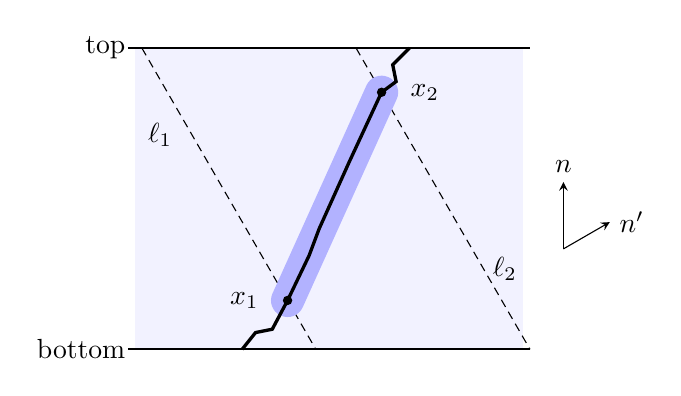
\begin{tikzpicture}[scale=.85,>=stealth]
 \fill[blue!5] (-1.5,0) rectangle (4.3,4.5);
 \draw[thick] (-1.6,0)--(4.4,0);
 \draw[thick] (-1.6,4.5)--(4.4,4.5);
 \node[left] at (-1.5,0) {bottom};
 \node[left] at (-1.5,4.5) {top};
 \coordinate (xone) at ({1.2-.73/sqrt(3)},.73);
 \coordinate (xtwo) at ({4.4-3.84/sqrt(3)},3.84);
 \draw[densely dashed] ({1.2-4.5/sqrt(3)},4.5)--(1.2,0);
 \draw[densely dashed] ({4.4-4.5/sqrt(3)},4.5)--(4.4,0);
 \draw[blue!30,line width=12pt,line cap=round]
        (xone)--(xtwo);
 \draw[very thick] (.1,0)--(.3,.25)--(.55,.3)--(xone);
 \draw[very thick] (xone)--(1.1,1.4)--(1.25,1.8)--(1.7,2.8)--(xtwo);
 \draw[very thick] (xtwo)--(2.4,4)--(2.35,4.25)--(2.6,4.5);
 \fill (xone) circle (2pt) node[left,xshift=-7pt] {$x_1$};
 \fill (xtwo) circle (2pt) node[right,xshift=7pt] {$x_2$};
 \draw[->] (4.9,1.5)--(4.9,2.5) node[above] {$n$};
 \draw[->] (4.9,1.5)--({4.9+.8*sqrt(3)/2},1.9) node[right] {$n'$};
 \node[left] at (-.8,3.2) {$\ell_1$};
 \node[right] at (3.7,1.2) {$\ell_2$};
\end{tikzpicture}
\caption{Changing the cut normal. The middle bridge follows a narrow
corridor between the tilted cuts $\ell_1,\ell_2$; the exterior pieces lie in separate
wedges. Each marked cut is crossed once. The diagram is schematic: the
thick lines indicate the three path pieces, not individual lattice edges.}
\label{a:tilted-corridor}
\end{figure}

Count the three-piece constructions modulo translations along the
bottom cut. In this quotient, the first crossing port $x_1$ has only
finitely many lattice residues at each permitted height, and there
are order $H$ such heights. Independently, the permitted interval
for $D$ contains order $H$ spacings. For each such port and gap, the
product of the three piece masses is at least a constant times
$H^{-3/4}$. Translate each resulting bottom endpoint to the prescribed root, retaining the two tilted cuts as
marks. The output with those marks recovers the crossing ports and
all three pieces, so this translation is bijective on the quotient.
If $K(\gamma)$ denotes the number of resulting marked representations
of the rooted output $\gamma$, then
\[
 \sum_\gamma w(\gamma)K(\gamma)\ge cH^{5/4}.
\]

For the second moment, take two representations of one output and
order their $k\le4$ distinct tilted cuts. The first is one of the
two first cuts and the last is one of the two second cuts; their
crossing ports therefore remain at distances comparable to $\delta H$
from the bottom and top, respectively. The rooted path starts before
every marked cut and finishes after every marked cut. Since each is
crossed exactly once, the crossings occur in the cut order, and the
intervening pieces stay in their open tilted slabs.

Again count modulo bottom translations. There are $O(H)$ choices
of the first crossing-port orbit. Reverse the first exterior piece:
its bottom endpoint is then free, and the wedge row bound sums that
endpoint with mass at most $CH^{-1/4}$. The last wedge has the same
uniform bound on its retained top-distance band. The original
junction diameters are $O(\delta H)$ and each original middle gap
is $O(H)$, so every spacing between consecutive cuts in the combined
list is at most $CH$. For each fixed spacing, intermediate crossing
ports are already summed by the total bridge mass $B_t$. Summing
positive spacings therefore costs at most
\[
 \sum_{1\le t\le CH}B_t\le C'H^{3/4}
\]
per internal layer. Keep the last-port distance restriction until
applying its uniform wedge bound, and drop the remaining restrictions
for an upper bound. Thus the contribution from $k$ distinct cuts is
at most
\[
 CH\,(H^{-1/4})^2(H^{3/4})^{k-1}
                      =CH^{-1/4+3k/4}.
\]
There are only finitely many ways to assign these cuts to the two
ordered mark pairs, including coincident cuts. Consequently
\[
 \sum_\gamma w(\gamma)K(\gamma)^2\le CH^{11/4}.
\]
Cauchy--Schwarz removes the marks and leaves total mass at least
\[
 \frac{(cH^{5/4})^2}{CH^{11/4}}=c'H^{-1/4}.
\]
All seam choices use their lattice spacings, which agree in physical
units by symmetry. Bounded rounding inside fixed positive relative
intervals changes only the constants.

From the straight corridor and this step we have guides at \(\pm60^\circ\) to any normal, hence also between them by mixtures. Transferring again from the appropriate tilted normal now covers any slope strictly forward on the original one. Concatenation as above gives the piecewise linear form. For uniformity, fix the tolerance $\varepsilon$ and cover the compact
family by finitely many uniform balls of radius $\varepsilon/3$ centered
at its graphs. Carry out the construction for each center with tolerance
$\varepsilon/3$, and take the minimum of the finitely many lower-bound
constants and the maximum of their lower height thresholds. Each
resulting corridor lies in the $\varepsilon$-corridor of any graph in its ball. This proves Theorem~\ref{a:bridge-spatial}.
